% Options for packages loaded elsewhere
% Options for packages loaded elsewhere
\PassOptionsToPackage{unicode}{hyperref}
\PassOptionsToPackage{hyphens}{url}
\PassOptionsToPackage{dvipsnames,svgnames,x11names}{xcolor}
%
\documentclass[
]{article}
\usepackage{xcolor}
\usepackage[margin=1in]{geometry}
\usepackage{amsmath,amssymb}
\setcounter{secnumdepth}{-\maxdimen} % remove section numbering
\usepackage{iftex}
\ifPDFTeX
  \usepackage[T1]{fontenc}
  \usepackage[utf8]{inputenc}
  \usepackage{textcomp} % provide euro and other symbols
\else % if luatex or xetex
  \usepackage{unicode-math} % this also loads fontspec
  \defaultfontfeatures{Scale=MatchLowercase}
  \defaultfontfeatures[\rmfamily]{Ligatures=TeX,Scale=1}
\fi
\usepackage{lmodern}
\ifPDFTeX\else
  % xetex/luatex font selection
\fi
% Use upquote if available, for straight quotes in verbatim environments
\IfFileExists{upquote.sty}{\usepackage{upquote}}{}
\IfFileExists{microtype.sty}{% use microtype if available
  \usepackage[]{microtype}
  \UseMicrotypeSet[protrusion]{basicmath} % disable protrusion for tt fonts
}{}
\makeatletter
\@ifundefined{KOMAClassName}{% if non-KOMA class
  \IfFileExists{parskip.sty}{%
    \usepackage{parskip}
  }{% else
    \setlength{\parindent}{0pt}
    \setlength{\parskip}{6pt plus 2pt minus 1pt}}
}{% if KOMA class
  \KOMAoptions{parskip=half}}
\makeatother
% Make \paragraph and \subparagraph free-standing
\makeatletter
\ifx\paragraph\undefined\else
  \let\oldparagraph\paragraph
  \renewcommand{\paragraph}{
    \@ifstar
      \xxxParagraphStar
      \xxxParagraphNoStar
  }
  \newcommand{\xxxParagraphStar}[1]{\oldparagraph*{#1}\mbox{}}
  \newcommand{\xxxParagraphNoStar}[1]{\oldparagraph{#1}\mbox{}}
\fi
\ifx\subparagraph\undefined\else
  \let\oldsubparagraph\subparagraph
  \renewcommand{\subparagraph}{
    \@ifstar
      \xxxSubParagraphStar
      \xxxSubParagraphNoStar
  }
  \newcommand{\xxxSubParagraphStar}[1]{\oldsubparagraph*{#1}\mbox{}}
  \newcommand{\xxxSubParagraphNoStar}[1]{\oldsubparagraph{#1}\mbox{}}
\fi
\makeatother

\usepackage{color}
\usepackage{fancyvrb}
\newcommand{\VerbBar}{|}
\newcommand{\VERB}{\Verb[commandchars=\\\{\}]}
\DefineVerbatimEnvironment{Highlighting}{Verbatim}{commandchars=\\\{\}}
% Add ',fontsize=\small' for more characters per line
\usepackage{framed}
\definecolor{shadecolor}{RGB}{241,243,245}
\newenvironment{Shaded}{\begin{snugshade}}{\end{snugshade}}
\newcommand{\AlertTok}[1]{\textcolor[rgb]{0.68,0.00,0.00}{#1}}
\newcommand{\AnnotationTok}[1]{\textcolor[rgb]{0.37,0.37,0.37}{#1}}
\newcommand{\AttributeTok}[1]{\textcolor[rgb]{0.40,0.45,0.13}{#1}}
\newcommand{\BaseNTok}[1]{\textcolor[rgb]{0.68,0.00,0.00}{#1}}
\newcommand{\BuiltInTok}[1]{\textcolor[rgb]{0.00,0.23,0.31}{#1}}
\newcommand{\CharTok}[1]{\textcolor[rgb]{0.13,0.47,0.30}{#1}}
\newcommand{\CommentTok}[1]{\textcolor[rgb]{0.37,0.37,0.37}{#1}}
\newcommand{\CommentVarTok}[1]{\textcolor[rgb]{0.37,0.37,0.37}{\textit{#1}}}
\newcommand{\ConstantTok}[1]{\textcolor[rgb]{0.56,0.35,0.01}{#1}}
\newcommand{\ControlFlowTok}[1]{\textcolor[rgb]{0.00,0.23,0.31}{\textbf{#1}}}
\newcommand{\DataTypeTok}[1]{\textcolor[rgb]{0.68,0.00,0.00}{#1}}
\newcommand{\DecValTok}[1]{\textcolor[rgb]{0.68,0.00,0.00}{#1}}
\newcommand{\DocumentationTok}[1]{\textcolor[rgb]{0.37,0.37,0.37}{\textit{#1}}}
\newcommand{\ErrorTok}[1]{\textcolor[rgb]{0.68,0.00,0.00}{#1}}
\newcommand{\ExtensionTok}[1]{\textcolor[rgb]{0.00,0.23,0.31}{#1}}
\newcommand{\FloatTok}[1]{\textcolor[rgb]{0.68,0.00,0.00}{#1}}
\newcommand{\FunctionTok}[1]{\textcolor[rgb]{0.28,0.35,0.67}{#1}}
\newcommand{\ImportTok}[1]{\textcolor[rgb]{0.00,0.46,0.62}{#1}}
\newcommand{\InformationTok}[1]{\textcolor[rgb]{0.37,0.37,0.37}{#1}}
\newcommand{\KeywordTok}[1]{\textcolor[rgb]{0.00,0.23,0.31}{\textbf{#1}}}
\newcommand{\NormalTok}[1]{\textcolor[rgb]{0.00,0.23,0.31}{#1}}
\newcommand{\OperatorTok}[1]{\textcolor[rgb]{0.37,0.37,0.37}{#1}}
\newcommand{\OtherTok}[1]{\textcolor[rgb]{0.00,0.23,0.31}{#1}}
\newcommand{\PreprocessorTok}[1]{\textcolor[rgb]{0.68,0.00,0.00}{#1}}
\newcommand{\RegionMarkerTok}[1]{\textcolor[rgb]{0.00,0.23,0.31}{#1}}
\newcommand{\SpecialCharTok}[1]{\textcolor[rgb]{0.37,0.37,0.37}{#1}}
\newcommand{\SpecialStringTok}[1]{\textcolor[rgb]{0.13,0.47,0.30}{#1}}
\newcommand{\StringTok}[1]{\textcolor[rgb]{0.13,0.47,0.30}{#1}}
\newcommand{\VariableTok}[1]{\textcolor[rgb]{0.07,0.07,0.07}{#1}}
\newcommand{\VerbatimStringTok}[1]{\textcolor[rgb]{0.13,0.47,0.30}{#1}}
\newcommand{\WarningTok}[1]{\textcolor[rgb]{0.37,0.37,0.37}{\textit{#1}}}

\usepackage{longtable,booktabs,array}
\newcounter{none} % for unnumbered tables
\usepackage{calc} % for calculating minipage widths
% Correct order of tables after \paragraph or \subparagraph
\usepackage{etoolbox}
\makeatletter
\patchcmd\longtable{\par}{\if@noskipsec\mbox{}\fi\par}{}{}
\makeatother
% Allow footnotes in longtable head/foot
\IfFileExists{footnotehyper.sty}{\usepackage{footnotehyper}}{\usepackage{footnote}}
\makesavenoteenv{longtable}
\usepackage{graphicx}
\makeatletter
\newsavebox\pandoc@box
\newcommand*\pandocbounded[1]{% scales image to fit in text height/width
  \sbox\pandoc@box{#1}%
  \Gscale@div\@tempa{\textheight}{\dimexpr\ht\pandoc@box+\dp\pandoc@box\relax}%
  \Gscale@div\@tempb{\linewidth}{\wd\pandoc@box}%
  \ifdim\@tempb\p@<\@tempa\p@\let\@tempa\@tempb\fi% select the smaller of both
  \ifdim\@tempa\p@<\p@\scalebox{\@tempa}{\usebox\pandoc@box}%
  \else\usebox{\pandoc@box}%
  \fi%
}
% Set default figure placement to htbp
\def\fps@figure{htbp}
\makeatother





\setlength{\emergencystretch}{3em} % prevent overfull lines

\providecommand{\tightlist}{%
  \setlength{\itemsep}{0pt}\setlength{\parskip}{0pt}}



 


% Shared LaTeX macros for 4SC000 slides and exercises.
% Starter set inferred from your existing PS1-PS3 notation (Bertsekas-style DP,
% LQR/Kalman, RL). Tell me what's wrong/missing when we get to lecture 1 and
% I'll fix it here once rather than slide-by-slide.
\newcommand{\E}{\mathbb{E}}
\newcommand{\Prob}{\text{Prob}}
\newcommand{\R}{\mathbb{R}}
\newcommand{\N}{\mathbb{N}}
\newcommand{\argmin}{\operatorname*{argmin}}
\newcommand{\argmax}{\operatorname*{argmax}}
\newcommand{\policy}{\mu}
\newcommand{\costtogo}{J}
\newcommand{\state}{x}
\newcommand{\action}{u}
\DeclareMathOperator*{\minimize}{minimize}
\makeatletter
\@ifpackageloaded{caption}{}{\usepackage{caption}}
\AtBeginDocument{%
\ifdefined\contentsname
  \renewcommand*\contentsname{Table of contents}
\else
  \newcommand\contentsname{Table of contents}
\fi
\ifdefined\listfigurename
  \renewcommand*\listfigurename{List of Figures}
\else
  \newcommand\listfigurename{List of Figures}
\fi
\ifdefined\listtablename
  \renewcommand*\listtablename{List of Tables}
\else
  \newcommand\listtablename{List of Tables}
\fi
\ifdefined\figurename
  \renewcommand*\figurename{Fig.}
\else
  \newcommand\figurename{Fig.}
\fi
\ifdefined\tablename
  \renewcommand*\tablename{Table}
\else
  \newcommand\tablename{Table}
\fi
}
\@ifpackageloaded{float}{}{\usepackage{float}}
\floatstyle{ruled}
\@ifundefined{c@chapter}{\newfloat{codelisting}{h}{lop}}{\newfloat{codelisting}{h}{lop}[chapter]}
\floatname{codelisting}{Listing}
\newcommand*\listoflistings{\listof{codelisting}{List of Listings}}
\makeatother
\makeatletter
\makeatother
\makeatletter
\@ifpackageloaded{caption}{}{\usepackage{caption}}
\@ifpackageloaded{subcaption}{}{\usepackage{subcaption}}
\makeatother
\usepackage{bookmark}
\IfFileExists{xurl.sty}{\usepackage{xurl}}{} % add URL line breaks if available
\urlstyle{same}
% fallback for those not using the hyperref driver hyperxmp:
\makeatletter
\@ifundefined{xmpquote}{\newcommand{\xmpquote}[1]{#1}}{}
\makeatother
\hypersetup{
  pdftitle={Robot path planning: deterministic vs stochastic},
  pdfauthor={Duarte Antunes},
  colorlinks=true,
  linkcolor={blue},
  filecolor={Maroon},
  citecolor={Blue},
  urlcolor={Blue},
  pdfcreator={LaTeX via pandoc}}


\title{Robot path planning: deterministic vs stochastic}
\author{Duarte Antunes}
\date{}
\begin{document}
\maketitle


The goal of this exercise is to understand the differences between
stochastic dynamic programming and dynamic programming for a simple
example where an agent/robot must move from left to right in a given
environment. For this example the environment in Figure 1 is considered.
The goal for the robot is to move from initial stage \(0\) to final
state \(h\) in minimum time.

\begin{figure}[t]

{\centering \pandocbounded{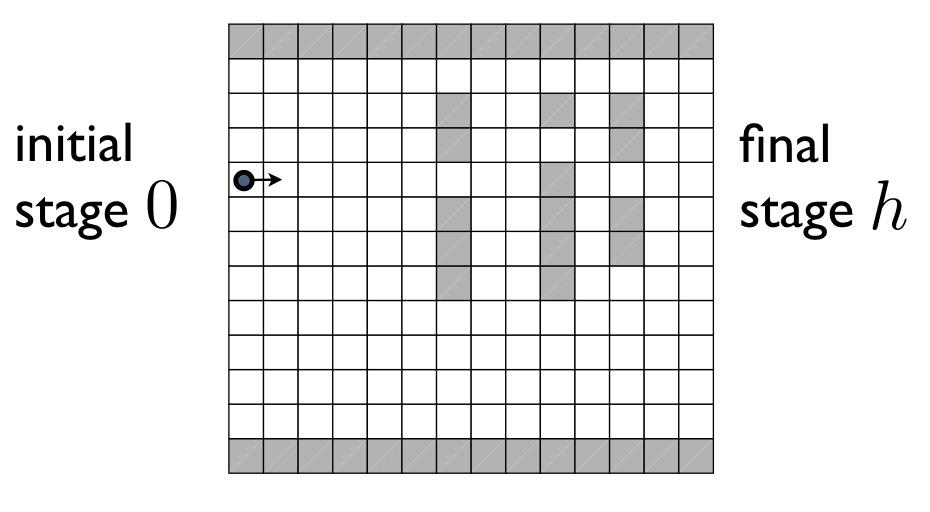
\includegraphics[keepaspectratio]{A_2_RobotPlanningStochastic_files/figure-pdf/cell-1-1-5966b484-8f0b-4379-bb5d-a90647b85d03.png}}

}

\caption{image\_0.png}

\end{figure}%

Figure 1: Considered environment

Let us start by considering a deterministic model according to the
following rules. If the robot is not stuck in an obstacle or in a wall
it can go up, straight or down. Otherwise, there is only one option (see
Figure 2). If the robot is not stuck in an obstacle or in a wall it can
go up, straight or down. Otherwise, there is only one option (see Figure
2). It takes I time unit to move horizontally from stage \(i\) to stage
\(i+1\) and \(\sqrt{2}\) time units to move diagonally. \(c\) time units
are paid every time an obstacle or a wall is hit.

\begin{figure}[t]

{\centering \pandocbounded{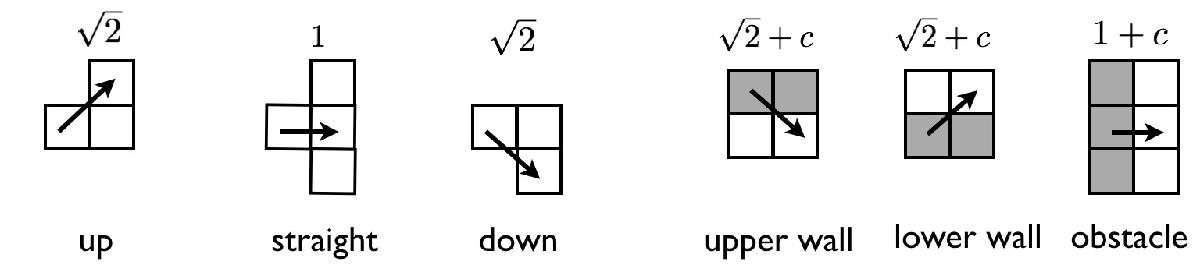
\includegraphics[keepaspectratio]{A_2_RobotPlanningStochastic_files/figure-pdf/cell-1-3-b6bfdf5f-4236-4074-99dc-4249b26477fb.png}}

}

\caption{image\_1.png}

\end{figure}%

Figure 2: Possible actions in the deterministic version

This problem can be written in the DP framework for a transition diagram
obtained from the rules of the problem, leading to the following
iteration for the costs-to-go:

for \(k=h\): \(J_h(i)=0\) for every \(i \in \{1,\dots,n\}\)

for \(k\in\{h-1,h-2,\dots,1,0\}\):

\$J\_\{k\}(1) =\sqrt{2}+c+J\_\{k+1\}(2) \$

\$ J\_\{k\}(n) =\sqrt{2}+c+J\_\{k+1\}(n-1)\$

and, for \(i\in\{2,\dots,n-1\}\),

\$ J\_\{k\}(i) =\min \left\{1+J\_\{k+1\}(i), \sqrt{2}+J\_\{k+1\}(i+1),
\sqrt{2}+J\_\{k+1\}(i-1)\right\}\$ (not an obstacle node)

\$J\_\{k\}(i) =1+c+J\_\{k+1\}(i) \$ (obstacle node)

Now assume that for regular nodes (no obstacles) the evolution of the
state is stochastic for every stage and state and the actions of the
robot have the stochastic behavior depicted in Figure 3

\begin{figure}[t]

{\centering \pandocbounded{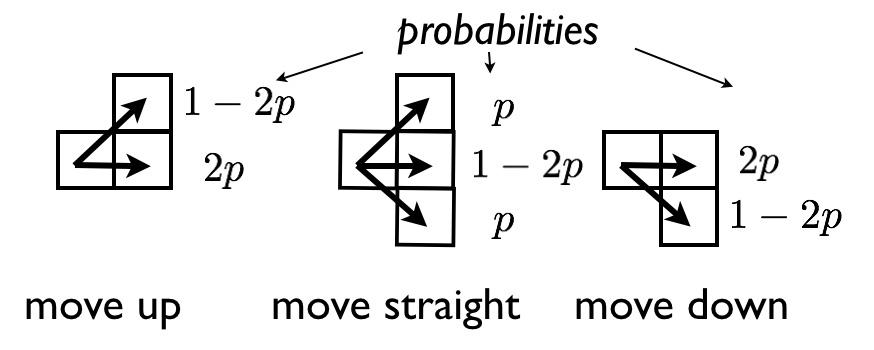
\includegraphics[keepaspectratio]{A_2_RobotPlanningStochastic_files/figure-pdf/cell-1-2-a6928c0e-c159-477c-920f-02b9e6cce6a7.png}}

}

\caption{image\_2.png}

\end{figure}%

Figure 3: Possible actions and outcomes in the stochastic version

Applying the stochastic dynamic programming algorithm leads now to the
equations

for \(k=h\): \(J_h(i)=0\) for every \(i \in \{1,\dots,n\}\)

for \(k\in\{h-1,h-2,\dots,1,0\}\):

\$J\_\{k\}(1) =\sqrt{2}+c+J\_\{k+1\}(2) \$

\(J_{k}(n) =\sqrt{2}+c+J_{k+1}(n-1)\)

and, for \(i\in\{2,\dots,n-1\}\),

\$J\_\{k\}(i)=\min \{(1-2
p)\left(1+J\_\{k+1\}(i)\right)+p\left(\sqrt{2}+J\_\{k+1\}(i+1)\right)+p\left(\sqrt{2}+J\_\{k+1\}(i-1)\right)
, \$

\(2 p\left(1+J_{k+1}(i)\right)+(1-2 p)\left(\sqrt{2}+J_{k+1}(i+1)\right) ,\)

\(2 p\left(1+J_{k+1}(i)\right)+(1-2 p)\left(\sqrt{2}+J_{k+1}(i-1)\right)\}\)
(not an obstable node)

\$J\_\{k\}(i) =1+c+J\_\{k+1\}(i) \$ (obstable node)

The following code provides and plots the optimal policy for both
deterministic and stochastic settings.

\begin{Shaded}
\begin{Highlighting}[]
\ImportTok{import}\NormalTok{ numpy }\ImportTok{as}\NormalTok{ np}
\ImportTok{import}\NormalTok{ matplotlib.pyplot }\ImportTok{as}\NormalTok{ plt}
\ImportTok{import}\NormalTok{ matplotlib.patches }\ImportTok{as}\NormalTok{ patches}

\NormalTok{np.set\_printoptions(precision }\OperatorTok{=} \DecValTok{4}\NormalTok{)}
\NormalTok{plt.rcParams[}\StringTok{"figure.figsize"}\NormalTok{] }\OperatorTok{=}\NormalTok{ (}\DecValTok{20}\NormalTok{, }\DecValTok{10}\NormalTok{)}
\end{Highlighting}
\end{Shaded}

\begin{Shaded}
\begin{Highlighting}[]
\KeywordTok{def}\NormalTok{ robotpathplanningBellman(M, c):}
\NormalTok{    [n, m] }\OperatorTok{=}\NormalTok{ M.shape}
\NormalTok{    J }\OperatorTok{=}\NormalTok{ np.zeros([n, m])}

\NormalTok{    u }\OperatorTok{=}\NormalTok{ [[[] }\ControlFlowTok{for}\NormalTok{ \_ }\KeywordTok{in} \BuiltInTok{range}\NormalTok{(n)] }\ControlFlowTok{for}\NormalTok{ \_ }\KeywordTok{in} \BuiltInTok{range}\NormalTok{(n)]}

    \ControlFlowTok{for}\NormalTok{ k }\KeywordTok{in} \BuiltInTok{range}\NormalTok{(m }\OperatorTok{{-}} \DecValTok{2}\NormalTok{, }\OperatorTok{{-}}\DecValTok{1}\NormalTok{, }\OperatorTok{{-}}\DecValTok{1}\NormalTok{):}
\NormalTok{        J[n }\OperatorTok{{-}} \DecValTok{1}\NormalTok{, k] }\OperatorTok{=}\NormalTok{ np.sqrt(}\DecValTok{2}\NormalTok{) }\OperatorTok{+}\NormalTok{ c }\OperatorTok{+}\NormalTok{ J[n }\OperatorTok{{-}} \DecValTok{2}\NormalTok{, k }\OperatorTok{+} \DecValTok{1}\NormalTok{]}
\NormalTok{        u[n }\OperatorTok{{-}} \DecValTok{1}\NormalTok{][k] }\OperatorTok{=} \DecValTok{3}      \CommentTok{\# "DOWN"}
\NormalTok{        J[}\DecValTok{0}\NormalTok{, k] }\OperatorTok{=}\NormalTok{ np.sqrt(}\DecValTok{2}\NormalTok{) }\OperatorTok{+}\NormalTok{ c }\OperatorTok{+}\NormalTok{ J[}\DecValTok{1}\NormalTok{, k }\OperatorTok{+} \DecValTok{1}\NormalTok{]}
\NormalTok{        u[}\DecValTok{0}\NormalTok{][k] }\OperatorTok{=} \DecValTok{2}          \CommentTok{\# "UP"}
        \ControlFlowTok{for}\NormalTok{ i }\KeywordTok{in} \BuiltInTok{range}\NormalTok{(}\DecValTok{1}\NormalTok{, n }\OperatorTok{{-}} \DecValTok{1}\NormalTok{):}
            \ControlFlowTok{if}\NormalTok{ M[i, k] }\OperatorTok{==} \DecValTok{0}\NormalTok{:}
\NormalTok{                J[i, k] }\OperatorTok{=} \DecValTok{1} \OperatorTok{+}\NormalTok{ c }\OperatorTok{+}\NormalTok{ J[i, k }\OperatorTok{+} \DecValTok{1}\NormalTok{]}
\NormalTok{                u[i][k] }\OperatorTok{=} \DecValTok{1}  \CommentTok{\# "STRAIGHT"}
            \ControlFlowTok{else}\NormalTok{:}
\NormalTok{                J[i, k] }\OperatorTok{=}\NormalTok{ np.}\BuiltInTok{min}\NormalTok{([}\DecValTok{1} \OperatorTok{+}\NormalTok{ J[i, k }\OperatorTok{+} \DecValTok{1}\NormalTok{], np.sqrt(}\DecValTok{2}\NormalTok{) }\OperatorTok{+}\NormalTok{ J[i }\OperatorTok{+} \DecValTok{1}\NormalTok{, k }\OperatorTok{+} \DecValTok{1}\NormalTok{], np.sqrt(}\DecValTok{2}\NormalTok{) }\OperatorTok{+}\NormalTok{ J[i }\OperatorTok{{-}} \DecValTok{1}\NormalTok{, k }\OperatorTok{+} \DecValTok{1}\NormalTok{]])}
\NormalTok{                dec }\OperatorTok{=}\NormalTok{ np.argmin([}\DecValTok{1} \OperatorTok{+}\NormalTok{ J[i, k }\OperatorTok{+} \DecValTok{1}\NormalTok{], np.sqrt(}\DecValTok{2}\NormalTok{) }\OperatorTok{+}\NormalTok{ J[i }\OperatorTok{+} \DecValTok{1}\NormalTok{, k }\OperatorTok{+} \DecValTok{1}\NormalTok{], np.sqrt(}\DecValTok{2}\NormalTok{) }\OperatorTok{+}\NormalTok{ J[i }\OperatorTok{{-}} \DecValTok{1}\NormalTok{, k }\OperatorTok{+} \DecValTok{1}\NormalTok{]])}
                \ControlFlowTok{if}\NormalTok{ dec }\OperatorTok{==} \DecValTok{0}\NormalTok{:}
\NormalTok{                    u[i][k] }\OperatorTok{=} \DecValTok{1}  \CommentTok{\# "STRAIGHT"}
                \ControlFlowTok{elif}\NormalTok{ dec }\OperatorTok{==} \DecValTok{1}\NormalTok{:}
\NormalTok{                    u[i][k] }\OperatorTok{=} \DecValTok{2}  \CommentTok{\# "UP"}
                \ControlFlowTok{elif}\NormalTok{ dec }\OperatorTok{==} \DecValTok{2}\NormalTok{:}
\NormalTok{                    u[i][k] }\OperatorTok{=} \DecValTok{3}  \CommentTok{\# "DOWN"}
    \ControlFlowTok{return}\NormalTok{ J, u}
\end{Highlighting}
\end{Shaded}

\begin{Shaded}
\begin{Highlighting}[]
\KeywordTok{def}\NormalTok{ stochasticrobotpathplanningBellman(M, c, p):}
\NormalTok{    [n, m] }\OperatorTok{=}\NormalTok{ M.shape}
\NormalTok{    J }\OperatorTok{=}\NormalTok{ np.zeros([n, m])}

\NormalTok{    u }\OperatorTok{=}\NormalTok{ [[[] }\ControlFlowTok{for}\NormalTok{ \_ }\KeywordTok{in} \BuiltInTok{range}\NormalTok{(n)] }\ControlFlowTok{for}\NormalTok{ \_ }\KeywordTok{in} \BuiltInTok{range}\NormalTok{(n)]}

    \ControlFlowTok{for}\NormalTok{ k }\KeywordTok{in} \BuiltInTok{range}\NormalTok{(m }\OperatorTok{{-}} \DecValTok{2}\NormalTok{, }\OperatorTok{{-}}\DecValTok{1}\NormalTok{, }\OperatorTok{{-}}\DecValTok{1}\NormalTok{):}
\NormalTok{        J[n }\OperatorTok{{-}} \DecValTok{1}\NormalTok{, k] }\OperatorTok{=}\NormalTok{ np.sqrt(}\DecValTok{2}\NormalTok{) }\OperatorTok{+}\NormalTok{ c }\OperatorTok{+}\NormalTok{ J[n }\OperatorTok{{-}} \DecValTok{2}\NormalTok{, k }\OperatorTok{+} \DecValTok{1}\NormalTok{]}
\NormalTok{        u[n }\OperatorTok{{-}} \DecValTok{1}\NormalTok{][k] }\OperatorTok{=} \DecValTok{3}       \CommentTok{\# "DOWN"}
\NormalTok{        J[}\DecValTok{0}\NormalTok{, k] }\OperatorTok{=}\NormalTok{ np.sqrt(}\DecValTok{2}\NormalTok{) }\OperatorTok{+}\NormalTok{ c }\OperatorTok{+}\NormalTok{ J[}\DecValTok{1}\NormalTok{, k }\OperatorTok{+} \DecValTok{1}\NormalTok{]}
\NormalTok{        u[}\DecValTok{0}\NormalTok{][k] }\OperatorTok{=} \DecValTok{2}           \CommentTok{\# "UP"}
        \ControlFlowTok{for}\NormalTok{ i }\KeywordTok{in} \BuiltInTok{range}\NormalTok{(}\DecValTok{1}\NormalTok{, n }\OperatorTok{{-}} \DecValTok{1}\NormalTok{):}
            \ControlFlowTok{if}\NormalTok{ M[i, k] }\OperatorTok{==} \DecValTok{0}\NormalTok{:}
\NormalTok{                J[i, k] }\OperatorTok{=} \DecValTok{1} \OperatorTok{+}\NormalTok{ c }\OperatorTok{+}\NormalTok{ J[i, k }\OperatorTok{+} \DecValTok{1}\NormalTok{]}

\NormalTok{                u[i][k] }\OperatorTok{=} \DecValTok{1}  \CommentTok{\# "STRAIGHT"}
            \ControlFlowTok{else}\NormalTok{:}
\NormalTok{                J[i, k] }\OperatorTok{=}\NormalTok{ np.}\BuiltInTok{min}\NormalTok{([(}\DecValTok{1} \OperatorTok{{-}} \DecValTok{2} \OperatorTok{*}\NormalTok{ p) }\OperatorTok{*}\NormalTok{ (}\DecValTok{1} \OperatorTok{+}\NormalTok{ J[i, k }\OperatorTok{+} \DecValTok{1}\NormalTok{]) }\OperatorTok{+}\NormalTok{ p }\OperatorTok{*}\NormalTok{ (np.sqrt(}\DecValTok{2}\NormalTok{) }\OperatorTok{+}\NormalTok{ J[i }\OperatorTok{+} \DecValTok{1}\NormalTok{, k }\OperatorTok{+} \DecValTok{1}\NormalTok{]) }\OperatorTok{+}\NormalTok{ p }\OperatorTok{*}\NormalTok{ (}
\NormalTok{                        np.sqrt(}\DecValTok{2}\NormalTok{) }\OperatorTok{+}\NormalTok{ J[i }\OperatorTok{{-}} \DecValTok{1}\NormalTok{, k }\OperatorTok{+} \DecValTok{1}\NormalTok{]),}
                                  \DecValTok{2} \OperatorTok{*}\NormalTok{ p }\OperatorTok{*}\NormalTok{ (}\DecValTok{1} \OperatorTok{+}\NormalTok{ J[i, k }\OperatorTok{+} \DecValTok{1}\NormalTok{]) }\OperatorTok{+}\NormalTok{ (}\DecValTok{1} \OperatorTok{{-}} \DecValTok{2} \OperatorTok{*}\NormalTok{ p) }\OperatorTok{*}\NormalTok{ (np.sqrt(}\DecValTok{2}\NormalTok{) }\OperatorTok{+}\NormalTok{ J[i }\OperatorTok{+} \DecValTok{1}\NormalTok{, k }\OperatorTok{+} \DecValTok{1}\NormalTok{]),}
                                  \DecValTok{2} \OperatorTok{*}\NormalTok{ p }\OperatorTok{*}\NormalTok{ (}\DecValTok{1} \OperatorTok{+}\NormalTok{ J[i, k }\OperatorTok{+} \DecValTok{1}\NormalTok{]) }\OperatorTok{+}\NormalTok{ (}\DecValTok{1} \OperatorTok{{-}} \DecValTok{2} \OperatorTok{*}\NormalTok{ p) }\OperatorTok{*}\NormalTok{ (np.sqrt(}\DecValTok{2}\NormalTok{) }\OperatorTok{+}\NormalTok{ J[i }\OperatorTok{{-}} \DecValTok{1}\NormalTok{, k }\OperatorTok{+} \DecValTok{1}\NormalTok{])])}

\NormalTok{                dec }\OperatorTok{=}\NormalTok{ np.argmin([(}\DecValTok{1} \OperatorTok{{-}} \DecValTok{2} \OperatorTok{*}\NormalTok{ p) }\OperatorTok{*}\NormalTok{ (}\DecValTok{1} \OperatorTok{+}\NormalTok{ J[i, k }\OperatorTok{+} \DecValTok{1}\NormalTok{]) }\OperatorTok{+}\NormalTok{ p }\OperatorTok{*}\NormalTok{ (np.sqrt(}\DecValTok{2}\NormalTok{) }\OperatorTok{+}\NormalTok{ J[i }\OperatorTok{+} \DecValTok{1}\NormalTok{, k }\OperatorTok{+} \DecValTok{1}\NormalTok{]) }\OperatorTok{+}\NormalTok{ p }\OperatorTok{*}\NormalTok{ (}
\NormalTok{                        np.sqrt(}\DecValTok{2}\NormalTok{) }\OperatorTok{+}\NormalTok{ J[i }\OperatorTok{{-}} \DecValTok{1}\NormalTok{, k }\OperatorTok{+} \DecValTok{1}\NormalTok{]),}
                                 \DecValTok{2} \OperatorTok{*}\NormalTok{ p }\OperatorTok{*}\NormalTok{ (}\DecValTok{1} \OperatorTok{+}\NormalTok{ J[i, k }\OperatorTok{+} \DecValTok{1}\NormalTok{]) }\OperatorTok{+}\NormalTok{ (}\DecValTok{1} \OperatorTok{{-}} \DecValTok{2} \OperatorTok{*}\NormalTok{ p) }\OperatorTok{*}\NormalTok{ (np.sqrt(}\DecValTok{2}\NormalTok{) }\OperatorTok{+}\NormalTok{ J[i }\OperatorTok{+} \DecValTok{1}\NormalTok{, k }\OperatorTok{+} \DecValTok{1}\NormalTok{]),}
                                 \DecValTok{2} \OperatorTok{*}\NormalTok{ p }\OperatorTok{*}\NormalTok{ (}\DecValTok{1} \OperatorTok{+}\NormalTok{ J[i, k }\OperatorTok{+} \DecValTok{1}\NormalTok{]) }\OperatorTok{+}\NormalTok{ (}\DecValTok{1} \OperatorTok{{-}} \DecValTok{2} \OperatorTok{*}\NormalTok{ p) }\OperatorTok{*}\NormalTok{ (np.sqrt(}\DecValTok{2}\NormalTok{) }\OperatorTok{+}\NormalTok{ J[i }\OperatorTok{{-}} \DecValTok{1}\NormalTok{, k }\OperatorTok{+} \DecValTok{1}\NormalTok{])])}
                \ControlFlowTok{if}\NormalTok{ dec }\OperatorTok{==} \DecValTok{0}\NormalTok{:}
\NormalTok{                    u[i][k] }\OperatorTok{=} \DecValTok{1}  \CommentTok{\# "STRAIGHT"}
                \ControlFlowTok{elif}\NormalTok{ dec }\OperatorTok{==} \DecValTok{1}\NormalTok{:}
\NormalTok{                    u[i][k] }\OperatorTok{=} \DecValTok{2}  \CommentTok{\# "UP"}
                \ControlFlowTok{elif}\NormalTok{ dec }\OperatorTok{==} \DecValTok{2}\NormalTok{:}
\NormalTok{                    u[i][k] }\OperatorTok{=} \DecValTok{3}  \CommentTok{\# "DOWN"}

    \ControlFlowTok{return}\NormalTok{ J, u}
\end{Highlighting}
\end{Shaded}

\begin{Shaded}
\begin{Highlighting}[]
\KeywordTok{def}\NormalTok{ plotsquare(l, r, ax, color):}
\NormalTok{    rect }\OperatorTok{=}\NormalTok{ patches.Rectangle((l, r), }\DecValTok{1}\NormalTok{, }\DecValTok{1}\NormalTok{, facecolor}\OperatorTok{=}\NormalTok{color, edgecolor}\OperatorTok{=}\StringTok{\textquotesingle{}k\textquotesingle{}}\NormalTok{)}
\NormalTok{    ax.add\_patch(rect)}
\end{Highlighting}
\end{Shaded}

\begin{Shaded}
\begin{Highlighting}[]
\KeywordTok{def}\NormalTok{ plottriangle(p, theta, ax):}
\NormalTok{    d1 }\OperatorTok{=} \FloatTok{0.30}
\NormalTok{    d2 }\OperatorTok{=} \FloatTok{0.06}
\NormalTok{    p1 }\OperatorTok{=}\NormalTok{ p}
\NormalTok{    p2 }\OperatorTok{=}\NormalTok{ p }\OperatorTok{+}\NormalTok{ np.array([}\OperatorTok{{-}}\NormalTok{d1 }\OperatorTok{*}\NormalTok{ np.cos(theta) }\OperatorTok{{-}}\NormalTok{ d2 }\OperatorTok{*}\NormalTok{ np.sin(theta), }
                       \OperatorTok{{-}}\NormalTok{d1 }\OperatorTok{*} \OperatorTok{{-}}\NormalTok{np.sin(theta) }\OperatorTok{{-}}\NormalTok{ d2 }\OperatorTok{*}\NormalTok{ np.cos(theta)])}
\NormalTok{    p3 }\OperatorTok{=}\NormalTok{ p }\OperatorTok{+}\NormalTok{ np.array([}\OperatorTok{{-}}\NormalTok{d1 }\OperatorTok{*}\NormalTok{ np.cos(theta) }\OperatorTok{+}\NormalTok{ d2 }\OperatorTok{*}\NormalTok{ np.sin(theta), }
                       \OperatorTok{{-}}\NormalTok{d1 }\OperatorTok{*} \OperatorTok{{-}}\NormalTok{np.sin(theta) }\OperatorTok{+}\NormalTok{ d2 }\OperatorTok{*}\NormalTok{ np.cos(theta)])}
\NormalTok{    tri }\OperatorTok{=}\NormalTok{ patches.Polygon(np.vstack([p3, p2, p1]), }\DecValTok{20}\NormalTok{, facecolor}\OperatorTok{=}\StringTok{\textquotesingle{}k\textquotesingle{}}\NormalTok{, edgecolor}\OperatorTok{=}\StringTok{\textquotesingle{}k\textquotesingle{}}\NormalTok{)}
\NormalTok{    ax.add\_patch(tri)}
\end{Highlighting}
\end{Shaded}

\begin{Shaded}
\begin{Highlighting}[]
\KeywordTok{def}\NormalTok{ plotpathplanning(J, M, u):}

\NormalTok{    n2 }\OperatorTok{=} \BuiltInTok{len}\NormalTok{(u)}
\NormalTok{    n1 }\OperatorTok{=} \BuiltInTok{len}\NormalTok{(u[}\DecValTok{0}\NormalTok{])}

\NormalTok{    action }\OperatorTok{=}\NormalTok{ [[[] }\ControlFlowTok{for}\NormalTok{ \_ }\KeywordTok{in} \BuiltInTok{range}\NormalTok{(n2)] }\ControlFlowTok{for}\NormalTok{ \_ }\KeywordTok{in} \BuiltInTok{range}\NormalTok{(n1 }\OperatorTok{{-}} \DecValTok{1}\NormalTok{)]}

    \ControlFlowTok{for}\NormalTok{ j }\KeywordTok{in} \BuiltInTok{range}\NormalTok{(}\DecValTok{0}\NormalTok{, n2):}
        \ControlFlowTok{for}\NormalTok{ i }\KeywordTok{in} \BuiltInTok{range}\NormalTok{(}\DecValTok{0}\NormalTok{, n1):}
            \ControlFlowTok{if}\NormalTok{ i }\OperatorTok{==} \DecValTok{0}\NormalTok{:}
\NormalTok{                action[}\DecValTok{0}\NormalTok{][j] }\OperatorTok{=}\NormalTok{ np.array([}\DecValTok{2}\NormalTok{, j }\OperatorTok{+} \DecValTok{1} \OperatorTok{+} \DecValTok{1}\NormalTok{])}
            \ControlFlowTok{else}\NormalTok{:}
                \ControlFlowTok{if}\NormalTok{ i }\OperatorTok{==}\NormalTok{ n1 }\OperatorTok{{-}} \DecValTok{1}\NormalTok{:}
\NormalTok{                    action[}\DecValTok{0}\NormalTok{][j] }\OperatorTok{=}\NormalTok{ np.array([n1 }\OperatorTok{{-}} \DecValTok{1}\NormalTok{, j }\OperatorTok{+} \DecValTok{1} \OperatorTok{+} \DecValTok{1}\NormalTok{])}

                \ControlFlowTok{else}\NormalTok{:}
                    \ControlFlowTok{if}\NormalTok{ u[i][j] }\OperatorTok{==} \DecValTok{1}\NormalTok{:}
\NormalTok{                        action[i][j] }\OperatorTok{=}\NormalTok{ np.array([i }\OperatorTok{+} \DecValTok{1}\NormalTok{, j }\OperatorTok{+} \DecValTok{1} \OperatorTok{+} \DecValTok{1}\NormalTok{])}

                    \ControlFlowTok{elif}\NormalTok{ u[i][j] }\OperatorTok{==} \DecValTok{2}\NormalTok{:}
\NormalTok{                        action[i][j] }\OperatorTok{=}\NormalTok{ np.array([i }\OperatorTok{+} \DecValTok{1} \OperatorTok{+} \DecValTok{1}\NormalTok{, j }\OperatorTok{+} \DecValTok{1} \OperatorTok{+} \DecValTok{1}\NormalTok{])}

                    \ControlFlowTok{else}\NormalTok{:}
\NormalTok{                        action[i][j] }\OperatorTok{=}\NormalTok{ np.array([i, j }\OperatorTok{+} \DecValTok{1} \OperatorTok{+} \DecValTok{1}\NormalTok{])}

\NormalTok{    [p, m] }\OperatorTok{=}\NormalTok{ M.shape}
\NormalTok{    deltapx }\OperatorTok{=} \FloatTok{0.2}
\NormalTok{    deltapy }\OperatorTok{=} \FloatTok{0.4}

\NormalTok{    fig, ax }\OperatorTok{=}\NormalTok{ plt.subplots(}\DecValTok{1}\NormalTok{)}
\NormalTok{    ax.set\_xlim(}\DecValTok{1}\NormalTok{, m }\OperatorTok{+} \DecValTok{1}\NormalTok{)}
\NormalTok{    ax.set\_ylim(}\DecValTok{1}\NormalTok{, p }\OperatorTok{+} \DecValTok{1}\NormalTok{)}

    \ControlFlowTok{for}\NormalTok{ r }\KeywordTok{in} \BuiltInTok{range}\NormalTok{(}\DecValTok{0}\NormalTok{, p):}
        \ControlFlowTok{for}\NormalTok{ l }\KeywordTok{in} \BuiltInTok{range}\NormalTok{(}\DecValTok{0}\NormalTok{, m):}
            \ControlFlowTok{if}\NormalTok{ M[r, l] }\OperatorTok{==} \DecValTok{0}\NormalTok{:}
\NormalTok{                plotsquare(l }\OperatorTok{+} \DecValTok{1}\NormalTok{, r }\OperatorTok{+} \DecValTok{1}\NormalTok{, ax, }\StringTok{\textquotesingle{}grey\textquotesingle{}}\NormalTok{)}
\NormalTok{                plt.text(l }\OperatorTok{+} \DecValTok{1} \OperatorTok{+}\NormalTok{ deltapx, r }\OperatorTok{+} \DecValTok{1} \OperatorTok{+}\NormalTok{ deltapy, }\StringTok{"}\SpecialCharTok{\%.2f}\StringTok{"}\OperatorTok{\%}\NormalTok{J[r, l], fontsize}\OperatorTok{=}\DecValTok{16}\NormalTok{)}
                
            \ControlFlowTok{else}\NormalTok{:}
\NormalTok{                plotsquare(l }\OperatorTok{+} \DecValTok{1}\NormalTok{, r }\OperatorTok{+} \DecValTok{1}\NormalTok{, ax, }\StringTok{\textquotesingle{}white\textquotesingle{}}\NormalTok{)}
\NormalTok{                plt.text(l }\OperatorTok{+} \DecValTok{1} \OperatorTok{+}\NormalTok{ deltapx, r }\OperatorTok{+} \DecValTok{1} \OperatorTok{+}\NormalTok{ deltapy, }\StringTok{"}\SpecialCharTok{\%.2f}\StringTok{"}\OperatorTok{\%}\NormalTok{J[r, l], fontsize}\OperatorTok{=}\DecValTok{16}\NormalTok{)}
  
\NormalTok{    fig, ax }\OperatorTok{=}\NormalTok{ plt.subplots(}\DecValTok{1}\NormalTok{)}
\NormalTok{    ax.set\_xlim(}\DecValTok{1}\NormalTok{, m }\OperatorTok{+} \DecValTok{1}\NormalTok{)}
\NormalTok{    ax.set\_ylim(}\DecValTok{1}\NormalTok{, p }\OperatorTok{+} \DecValTok{1}\NormalTok{)}

    \ControlFlowTok{for}\NormalTok{ r }\KeywordTok{in} \BuiltInTok{range}\NormalTok{(}\DecValTok{0}\NormalTok{, p):}
        \ControlFlowTok{for}\NormalTok{ l }\KeywordTok{in} \BuiltInTok{range}\NormalTok{(}\DecValTok{0}\NormalTok{, m }\OperatorTok{{-}} \DecValTok{1}\NormalTok{):}
            \ControlFlowTok{if}\NormalTok{ M[r, l] }\OperatorTok{==} \DecValTok{0}\NormalTok{:}
\NormalTok{                plotsquare(l }\OperatorTok{+} \DecValTok{1}\NormalTok{, r }\OperatorTok{+} \DecValTok{1}\NormalTok{, ax, }\StringTok{\textquotesingle{}grey\textquotesingle{}}\NormalTok{)}
                
                \ControlFlowTok{if} \VariableTok{True}\NormalTok{:}
                    \ControlFlowTok{if}\NormalTok{ r }\OperatorTok{==} \DecValTok{0}\NormalTok{:}
\NormalTok{                        ax.plot([l }\OperatorTok{+} \DecValTok{1} \OperatorTok{+} \FloatTok{0.25}\NormalTok{, l }\OperatorTok{+} \DecValTok{1} \OperatorTok{+} \FloatTok{0.75}\NormalTok{], [r }\OperatorTok{+} \DecValTok{1} \OperatorTok{+} \FloatTok{0.25}\NormalTok{, r }\OperatorTok{+} \DecValTok{1} \OperatorTok{+} \FloatTok{0.75}\NormalTok{], }\StringTok{\textquotesingle{}k\textquotesingle{}}\NormalTok{)}
\NormalTok{                        plottriangle(np.array([l }\OperatorTok{+} \DecValTok{1} \OperatorTok{+} \FloatTok{0.75}\NormalTok{, r }\OperatorTok{+} \DecValTok{1} \OperatorTok{+} \FloatTok{0.75}\NormalTok{]), }\OperatorTok{{-}}\NormalTok{np.pi }\OperatorTok{/} \DecValTok{4}\NormalTok{, ax)}
                        
                    \ControlFlowTok{else}\NormalTok{:}
                        \ControlFlowTok{if}\NormalTok{ r }\OperatorTok{==}\NormalTok{ p }\OperatorTok{{-}} \DecValTok{1}\NormalTok{:}
\NormalTok{                            ax.plot([l }\OperatorTok{+} \DecValTok{1} \OperatorTok{+} \FloatTok{0.25}\NormalTok{, l }\OperatorTok{+} \DecValTok{1} \OperatorTok{+} \FloatTok{0.75}\NormalTok{], [r }\OperatorTok{+} \DecValTok{1} \OperatorTok{+} \FloatTok{0.75}\NormalTok{, r }\OperatorTok{+} \DecValTok{1} \OperatorTok{+} \FloatTok{0.25}\NormalTok{], }\StringTok{\textquotesingle{}k\textquotesingle{}}\NormalTok{)}
\NormalTok{                            plottriangle(np.array([l }\OperatorTok{+} \DecValTok{1} \OperatorTok{+} \FloatTok{0.75}\NormalTok{, r }\OperatorTok{+} \DecValTok{1} \OperatorTok{+} \FloatTok{0.25}\NormalTok{]), np.pi }\OperatorTok{/} \DecValTok{4}\NormalTok{, ax)}
                            
                        \ControlFlowTok{else}\NormalTok{:}
\NormalTok{                            ax.plot([l }\OperatorTok{+} \DecValTok{1} \OperatorTok{+} \FloatTok{0.25}\NormalTok{, l }\OperatorTok{+} \DecValTok{1} \OperatorTok{+} \FloatTok{0.75}\NormalTok{], [r }\OperatorTok{+} \DecValTok{1} \OperatorTok{+} \FloatTok{0.5}\NormalTok{, r }\OperatorTok{+} \DecValTok{1} \OperatorTok{+} \FloatTok{0.5}\NormalTok{], }\StringTok{\textquotesingle{}k\textquotesingle{}}\NormalTok{)}
\NormalTok{                            plottriangle(np.array([l }\OperatorTok{+} \DecValTok{1} \OperatorTok{+} \FloatTok{0.75}\NormalTok{, r }\OperatorTok{+} \DecValTok{1} \OperatorTok{+} \FloatTok{0.5}\NormalTok{]), }\DecValTok{0}\NormalTok{, ax)}
                            

            \ControlFlowTok{else}\NormalTok{:}
\NormalTok{                plotsquare(l }\OperatorTok{+} \DecValTok{1}\NormalTok{, r }\OperatorTok{+} \DecValTok{1}\NormalTok{, ax, }\StringTok{\textquotesingle{}white\textquotesingle{}}\NormalTok{)}
                
\NormalTok{                actionrl }\OperatorTok{=}\NormalTok{ np.array2string(action[r][l] }\OperatorTok{{-}}\NormalTok{ [r }\OperatorTok{+} \DecValTok{1}\NormalTok{, l }\OperatorTok{+} \DecValTok{1}\NormalTok{])}
                                
                \ControlFlowTok{if}\NormalTok{ actionrl }\OperatorTok{==}\NormalTok{ np.array2string(np.array([}\DecValTok{0}\NormalTok{, }\DecValTok{0}\NormalTok{])):}
                    \ControlFlowTok{continue}

                \ControlFlowTok{elif}\NormalTok{ actionrl }\OperatorTok{==}\NormalTok{ np.array2string(np.array([}\OperatorTok{{-}}\DecValTok{1}\NormalTok{, }\DecValTok{1}\NormalTok{])):}
\NormalTok{                    ax.plot([l }\OperatorTok{+} \DecValTok{1} \OperatorTok{+} \FloatTok{0.25}\NormalTok{, l }\OperatorTok{+} \DecValTok{1} \OperatorTok{+} \FloatTok{0.75}\NormalTok{], [r }\OperatorTok{+} \DecValTok{1} \OperatorTok{+} \FloatTok{0.75}\NormalTok{, r }\OperatorTok{+} \DecValTok{1} \OperatorTok{+} \FloatTok{0.25}\NormalTok{], }\StringTok{\textquotesingle{}k\textquotesingle{}}\NormalTok{)}
\NormalTok{                    plottriangle(np.array([l }\OperatorTok{+} \DecValTok{1} \OperatorTok{+} \FloatTok{0.75}\NormalTok{, r }\OperatorTok{+} \DecValTok{1} \OperatorTok{+} \FloatTok{0.25}\NormalTok{]), np.pi }\OperatorTok{/} \DecValTok{4}\NormalTok{, ax)}

                \ControlFlowTok{elif}\NormalTok{ actionrl }\OperatorTok{==}\NormalTok{ np.array2string(np.array([}\OperatorTok{{-}}\DecValTok{1}\NormalTok{, }\DecValTok{0}\NormalTok{])):}
\NormalTok{                    ax.plot([l }\OperatorTok{+} \DecValTok{1} \OperatorTok{+} \FloatTok{0.5}\NormalTok{, l }\OperatorTok{+} \DecValTok{1} \OperatorTok{+} \FloatTok{0.5}\NormalTok{], [r }\OperatorTok{+} \DecValTok{1} \OperatorTok{+} \FloatTok{0.25}\NormalTok{, r }\OperatorTok{+} \DecValTok{1} \OperatorTok{+} \FloatTok{0.75}\NormalTok{], }\StringTok{\textquotesingle{}k\textquotesingle{}}\NormalTok{)}
\NormalTok{                    plottriangle(np.array([l }\OperatorTok{+} \DecValTok{1} \OperatorTok{+} \FloatTok{0.5}\NormalTok{, r }\OperatorTok{+} \DecValTok{1} \OperatorTok{+} \FloatTok{0.25}\NormalTok{]), np.pi }\OperatorTok{/} \DecValTok{2}\NormalTok{, ax)}

                \ControlFlowTok{elif}\NormalTok{ actionrl }\OperatorTok{==}\NormalTok{ np.array2string(np.array([}\OperatorTok{{-}}\DecValTok{1}\NormalTok{, }\OperatorTok{{-}}\DecValTok{1}\NormalTok{])):}
\NormalTok{                    ax.plot([l }\OperatorTok{+} \DecValTok{1} \OperatorTok{+} \FloatTok{0.25}\NormalTok{, l }\OperatorTok{+} \DecValTok{1} \OperatorTok{+} \FloatTok{0.75}\NormalTok{], [r }\OperatorTok{+} \DecValTok{1} \OperatorTok{+} \FloatTok{0.25}\NormalTok{, r }\OperatorTok{+} \DecValTok{1} \OperatorTok{+} \FloatTok{0.75}\NormalTok{], }\StringTok{\textquotesingle{}k\textquotesingle{}}\NormalTok{)}
\NormalTok{                    plottriangle(np.array([l }\OperatorTok{+} \DecValTok{1} \OperatorTok{+} \FloatTok{0.25}\NormalTok{, r }\OperatorTok{+} \DecValTok{1} \OperatorTok{+} \FloatTok{0.25}\NormalTok{]), }\DecValTok{3}\OperatorTok{*}\NormalTok{np.pi }\OperatorTok{/} \DecValTok{4}\NormalTok{, ax)}

                \ControlFlowTok{elif}\NormalTok{ actionrl }\OperatorTok{==}\NormalTok{ np.array2string(np.array([}\DecValTok{0}\NormalTok{, }\OperatorTok{{-}}\DecValTok{1}\NormalTok{])):}
\NormalTok{                    ax.plot([l }\OperatorTok{+} \DecValTok{1} \OperatorTok{+} \FloatTok{0.25}\NormalTok{, l }\OperatorTok{+} \DecValTok{1} \OperatorTok{+} \FloatTok{0.75}\NormalTok{], [r }\OperatorTok{+} \DecValTok{1} \OperatorTok{+} \FloatTok{0.5}\NormalTok{, r }\OperatorTok{+} \DecValTok{1} \OperatorTok{+} \FloatTok{0.5}\NormalTok{], }\StringTok{\textquotesingle{}k\textquotesingle{}}\NormalTok{)}
\NormalTok{                    plottriangle(np.array([l }\OperatorTok{+} \DecValTok{1} \OperatorTok{+} \FloatTok{0.25}\NormalTok{, r }\OperatorTok{+} \DecValTok{1} \OperatorTok{+} \FloatTok{0.5}\NormalTok{]), np.pi, ax)}

                \ControlFlowTok{elif}\NormalTok{ actionrl }\OperatorTok{==}\NormalTok{ np.array2string(np.array([}\DecValTok{1}\NormalTok{, }\OperatorTok{{-}}\DecValTok{1}\NormalTok{])):}
\NormalTok{                    ax.plot([l }\OperatorTok{+} \DecValTok{1} \OperatorTok{+} \FloatTok{0.25}\NormalTok{, l }\OperatorTok{+} \DecValTok{1} \OperatorTok{+} \FloatTok{0.75}\NormalTok{], [r }\OperatorTok{+} \DecValTok{1} \OperatorTok{+} \FloatTok{0.75}\NormalTok{, r }\OperatorTok{+} \DecValTok{1} \OperatorTok{+} \FloatTok{0.25}\NormalTok{], }\StringTok{\textquotesingle{}k\textquotesingle{}}\NormalTok{)}
\NormalTok{                    plottriangle(np.array([l }\OperatorTok{+} \DecValTok{1} \OperatorTok{+} \FloatTok{0.25}\NormalTok{, r }\OperatorTok{+} \DecValTok{1} \OperatorTok{+} \FloatTok{0.75}\NormalTok{]), }\OperatorTok{{-}}\DecValTok{3} \OperatorTok{*}\NormalTok{ np.pi }\OperatorTok{/} \DecValTok{4}\NormalTok{, ax)}

                \ControlFlowTok{elif}\NormalTok{ actionrl }\OperatorTok{==}\NormalTok{ np.array2string(np.array([}\DecValTok{1}\NormalTok{, }\DecValTok{0}\NormalTok{])):}
\NormalTok{                    ax.plot([l }\OperatorTok{+} \DecValTok{1} \OperatorTok{+} \FloatTok{0.5}\NormalTok{, l }\OperatorTok{+} \DecValTok{1} \OperatorTok{+} \FloatTok{0.5}\NormalTok{], [r }\OperatorTok{+} \DecValTok{1} \OperatorTok{+} \FloatTok{0.25}\NormalTok{, r }\OperatorTok{+} \DecValTok{1} \OperatorTok{+} \FloatTok{0.75}\NormalTok{], }\StringTok{\textquotesingle{}k\textquotesingle{}}\NormalTok{)}
\NormalTok{                    plottriangle(np.array([l }\OperatorTok{+} \DecValTok{1} \OperatorTok{+} \FloatTok{0.5}\NormalTok{, r }\OperatorTok{+} \DecValTok{1} \OperatorTok{+} \FloatTok{0.75}\NormalTok{]), }\OperatorTok{{-}}\NormalTok{np.pi }\OperatorTok{/} \DecValTok{2}\NormalTok{, ax)}

                \ControlFlowTok{elif}\NormalTok{ actionrl }\OperatorTok{==}\NormalTok{ np.array2string(np.array([}\DecValTok{1}\NormalTok{, }\DecValTok{1}\NormalTok{])):}
\NormalTok{                    ax.plot([l }\OperatorTok{+} \DecValTok{1} \OperatorTok{+} \FloatTok{0.25}\NormalTok{, l }\OperatorTok{+} \DecValTok{1} \OperatorTok{+} \FloatTok{0.75}\NormalTok{], [r }\OperatorTok{+} \DecValTok{1} \OperatorTok{+} \FloatTok{0.25}\NormalTok{, r }\OperatorTok{+} \DecValTok{1} \OperatorTok{+} \FloatTok{0.75}\NormalTok{], }\StringTok{\textquotesingle{}k\textquotesingle{}}\NormalTok{)}
\NormalTok{                    plottriangle(np.array([l }\OperatorTok{+} \DecValTok{1} \OperatorTok{+} \FloatTok{0.75}\NormalTok{, r }\OperatorTok{+} \DecValTok{1} \OperatorTok{+} \FloatTok{0.75}\NormalTok{]), }\OperatorTok{{-}}\NormalTok{np.pi }\OperatorTok{/} \DecValTok{4}\NormalTok{, ax)}

                \ControlFlowTok{elif}\NormalTok{ actionrl }\OperatorTok{==}\NormalTok{ np.array2string(np.array([}\DecValTok{0}\NormalTok{, }\DecValTok{1}\NormalTok{])):}
\NormalTok{                    ax.plot([l }\OperatorTok{+} \DecValTok{1} \OperatorTok{+} \FloatTok{0.25}\NormalTok{, l }\OperatorTok{+} \DecValTok{1} \OperatorTok{+} \FloatTok{0.75}\NormalTok{], [r }\OperatorTok{+} \DecValTok{1} \OperatorTok{+} \FloatTok{0.5}\NormalTok{, r }\OperatorTok{+} \DecValTok{1} \OperatorTok{+} \FloatTok{0.5}\NormalTok{], }\StringTok{\textquotesingle{}k\textquotesingle{}}\NormalTok{)}
\NormalTok{                    plottriangle(np.array([l }\OperatorTok{+} \DecValTok{1} \OperatorTok{+} \FloatTok{0.75}\NormalTok{, r }\OperatorTok{+} \DecValTok{1} \OperatorTok{+} \FloatTok{0.5}\NormalTok{]), }\DecValTok{0}\NormalTok{, ax)}


    \ControlFlowTok{return}
\end{Highlighting}
\end{Shaded}

\begin{Shaded}
\begin{Highlighting}[]
\NormalTok{M }\OperatorTok{=}\NormalTok{ np.array([[}\DecValTok{0}\NormalTok{, }\DecValTok{0}\NormalTok{, }\DecValTok{0}\NormalTok{, }\DecValTok{0}\NormalTok{, }\DecValTok{0}\NormalTok{, }\DecValTok{0}\NormalTok{, }\DecValTok{0}\NormalTok{, }\DecValTok{0}\NormalTok{, }\DecValTok{0}\NormalTok{, }\DecValTok{0}\NormalTok{, }\DecValTok{0}\NormalTok{, }\DecValTok{0}\NormalTok{, }\DecValTok{0}\NormalTok{, }\DecValTok{0}\NormalTok{],}
\NormalTok{              [}\DecValTok{1}\NormalTok{, }\DecValTok{1}\NormalTok{, }\DecValTok{1}\NormalTok{, }\DecValTok{1}\NormalTok{, }\DecValTok{1}\NormalTok{, }\DecValTok{1}\NormalTok{, }\DecValTok{1}\NormalTok{, }\DecValTok{1}\NormalTok{, }\DecValTok{1}\NormalTok{, }\DecValTok{1}\NormalTok{, }\DecValTok{1}\NormalTok{, }\DecValTok{1}\NormalTok{, }\DecValTok{1}\NormalTok{, }\DecValTok{1}\NormalTok{],}
\NormalTok{              [}\DecValTok{1}\NormalTok{, }\DecValTok{1}\NormalTok{, }\DecValTok{1}\NormalTok{, }\DecValTok{1}\NormalTok{, }\DecValTok{1}\NormalTok{, }\DecValTok{1}\NormalTok{, }\DecValTok{1}\NormalTok{, }\DecValTok{1}\NormalTok{, }\DecValTok{1}\NormalTok{, }\DecValTok{1}\NormalTok{, }\DecValTok{1}\NormalTok{, }\DecValTok{1}\NormalTok{, }\DecValTok{1}\NormalTok{, }\DecValTok{1}\NormalTok{],}
\NormalTok{              [}\DecValTok{1}\NormalTok{, }\DecValTok{1}\NormalTok{, }\DecValTok{1}\NormalTok{, }\DecValTok{1}\NormalTok{, }\DecValTok{1}\NormalTok{, }\DecValTok{1}\NormalTok{, }\DecValTok{1}\NormalTok{, }\DecValTok{1}\NormalTok{, }\DecValTok{1}\NormalTok{, }\DecValTok{1}\NormalTok{, }\DecValTok{1}\NormalTok{, }\DecValTok{1}\NormalTok{, }\DecValTok{1}\NormalTok{, }\DecValTok{1}\NormalTok{],}
\NormalTok{              [}\DecValTok{1}\NormalTok{, }\DecValTok{1}\NormalTok{, }\DecValTok{1}\NormalTok{, }\DecValTok{1}\NormalTok{, }\DecValTok{1}\NormalTok{, }\DecValTok{1}\NormalTok{, }\DecValTok{1}\NormalTok{, }\DecValTok{1}\NormalTok{, }\DecValTok{1}\NormalTok{, }\DecValTok{1}\NormalTok{, }\DecValTok{1}\NormalTok{, }\DecValTok{1}\NormalTok{, }\DecValTok{1}\NormalTok{, }\DecValTok{1}\NormalTok{],}
\NormalTok{              [}\DecValTok{1}\NormalTok{, }\DecValTok{1}\NormalTok{, }\DecValTok{1}\NormalTok{, }\DecValTok{1}\NormalTok{, }\DecValTok{1}\NormalTok{, }\DecValTok{1}\NormalTok{, }\DecValTok{0}\NormalTok{, }\DecValTok{1}\NormalTok{, }\DecValTok{1}\NormalTok{, }\DecValTok{0}\NormalTok{, }\DecValTok{1}\NormalTok{, }\DecValTok{1}\NormalTok{, }\DecValTok{1}\NormalTok{, }\DecValTok{1}\NormalTok{],}
\NormalTok{              [}\DecValTok{1}\NormalTok{, }\DecValTok{1}\NormalTok{, }\DecValTok{1}\NormalTok{, }\DecValTok{1}\NormalTok{, }\DecValTok{1}\NormalTok{, }\DecValTok{1}\NormalTok{, }\DecValTok{0}\NormalTok{, }\DecValTok{1}\NormalTok{, }\DecValTok{1}\NormalTok{, }\DecValTok{0}\NormalTok{, }\DecValTok{1}\NormalTok{, }\DecValTok{0}\NormalTok{, }\DecValTok{1}\NormalTok{, }\DecValTok{1}\NormalTok{],}
\NormalTok{              [}\DecValTok{1}\NormalTok{, }\DecValTok{1}\NormalTok{, }\DecValTok{1}\NormalTok{, }\DecValTok{1}\NormalTok{, }\DecValTok{1}\NormalTok{, }\DecValTok{1}\NormalTok{, }\DecValTok{0}\NormalTok{, }\DecValTok{1}\NormalTok{, }\DecValTok{1}\NormalTok{, }\DecValTok{0}\NormalTok{, }\DecValTok{1}\NormalTok{, }\DecValTok{0}\NormalTok{, }\DecValTok{1}\NormalTok{, }\DecValTok{1}\NormalTok{],}
\NormalTok{              [}\DecValTok{1}\NormalTok{, }\DecValTok{1}\NormalTok{, }\DecValTok{1}\NormalTok{, }\DecValTok{1}\NormalTok{, }\DecValTok{1}\NormalTok{, }\DecValTok{1}\NormalTok{, }\DecValTok{1}\NormalTok{, }\DecValTok{1}\NormalTok{, }\DecValTok{1}\NormalTok{, }\DecValTok{0}\NormalTok{, }\DecValTok{1}\NormalTok{, }\DecValTok{1}\NormalTok{, }\DecValTok{1}\NormalTok{, }\DecValTok{1}\NormalTok{],}
\NormalTok{              [}\DecValTok{1}\NormalTok{, }\DecValTok{1}\NormalTok{, }\DecValTok{1}\NormalTok{, }\DecValTok{1}\NormalTok{, }\DecValTok{1}\NormalTok{, }\DecValTok{1}\NormalTok{, }\DecValTok{0}\NormalTok{, }\DecValTok{1}\NormalTok{, }\DecValTok{1}\NormalTok{, }\DecValTok{1}\NormalTok{, }\DecValTok{1}\NormalTok{, }\DecValTok{0}\NormalTok{, }\DecValTok{1}\NormalTok{, }\DecValTok{1}\NormalTok{],}
\NormalTok{              [}\DecValTok{1}\NormalTok{, }\DecValTok{1}\NormalTok{, }\DecValTok{1}\NormalTok{, }\DecValTok{1}\NormalTok{, }\DecValTok{1}\NormalTok{, }\DecValTok{1}\NormalTok{, }\DecValTok{0}\NormalTok{, }\DecValTok{1}\NormalTok{, }\DecValTok{1}\NormalTok{, }\DecValTok{0}\NormalTok{, }\DecValTok{1}\NormalTok{, }\DecValTok{0}\NormalTok{, }\DecValTok{1}\NormalTok{, }\DecValTok{1}\NormalTok{],}
\NormalTok{              [}\DecValTok{1}\NormalTok{, }\DecValTok{1}\NormalTok{, }\DecValTok{1}\NormalTok{, }\DecValTok{1}\NormalTok{, }\DecValTok{1}\NormalTok{, }\DecValTok{1}\NormalTok{, }\DecValTok{1}\NormalTok{, }\DecValTok{1}\NormalTok{, }\DecValTok{1}\NormalTok{, }\DecValTok{1}\NormalTok{, }\DecValTok{1}\NormalTok{, }\DecValTok{1}\NormalTok{, }\DecValTok{1}\NormalTok{, }\DecValTok{1}\NormalTok{],}
\NormalTok{              [}\DecValTok{0}\NormalTok{, }\DecValTok{0}\NormalTok{, }\DecValTok{0}\NormalTok{, }\DecValTok{0}\NormalTok{, }\DecValTok{0}\NormalTok{, }\DecValTok{0}\NormalTok{, }\DecValTok{0}\NormalTok{, }\DecValTok{0}\NormalTok{, }\DecValTok{0}\NormalTok{, }\DecValTok{0}\NormalTok{, }\DecValTok{0}\NormalTok{, }\DecValTok{0}\NormalTok{, }\DecValTok{0}\NormalTok{, }\DecValTok{0}\NormalTok{]])}

\NormalTok{c }\OperatorTok{=} \DecValTok{4}
\NormalTok{p }\OperatorTok{=} \FloatTok{0.1}

\NormalTok{[Jdet, udet] }\OperatorTok{=}\NormalTok{ robotpathplanningBellman(M, c)}
\end{Highlighting}
\end{Shaded}

\begin{Shaded}
\begin{Highlighting}[]
\NormalTok{[J, u] }\OperatorTok{=}\NormalTok{ stochasticrobotpathplanningBellman(M, c, p)}
\end{Highlighting}
\end{Shaded}

\begin{Shaded}
\begin{Highlighting}[]
\NormalTok{plotpathplanning(Jdet, M, udet)}
\end{Highlighting}
\end{Shaded}

\begin{Shaded}
\begin{Highlighting}[]
\NormalTok{plotpathplanning(J, M, u)}
\end{Highlighting}
\end{Shaded}





\end{document}
